\chapter{Una teoría de la memoria para secuencias binarias: evidencia de un algoritmo de compresión mental en humanos}

\section{Introducción}

%Sequence processing, the ability to encode and represent in memory a temporally ordered series of discrete elements, plays a central role in numerous human activities, including language. In the 1950’s, Karl Lashley (1) and Noam Chomsky (2) famously argued that the sequential structures that humans produce and remember cannot be reduced to mere associations of consecutive items, as envisaged in the associative theories characteristic of the Skinnerian paradigm, but must be mentally represented as recursively nested structures. The syntax of language, for instance, involves a recursive grammar of potentially unlimited embeddings of phrases within phrases, and a similar argument has been made for a “musical grammar” (3). Here, we formulate and test the theory that a similar code is needed to account for the much simpler case of binary sequences, i.e. sequences composed of two items A and B (e.g. high and low pitch tones, or red and green dots). We present experimental evidence that, even in this simple case, which can be considered as the simplest possible form of “music”, a similar postulation of nested structures is required in order to account for human memory performance. 

El procesamiento de secuencias, la capacidad de codificar y representar en la memoria una serie de elementos discretos ordenados temporalmente, juega un papel central en numerosas actividades humanas, incluido el lenguaje. En la década de 1950, Karl Lashley \cite{f1} y Noam Chomsky \cite{f2} argumentaron que las estructuras secuenciales que los humanos producen y recuerdan no pueden reducirse a meras asociaciones de elementos consecutivos, como se prevé en las teorías asociativas típicas del paradigma Skinneriano, sino que deben ser representadas mentalmente como estructuras recursivamente anidadas. La sintaxis del lenguaje, por ejemplo, implica una gramática recursiva con potencialmente infinitas inserciones de frases dentro de frases, y un argumento similar se ha propuesto para la \textit{gramática musical} \cite{f3}. En este capítulo, formulamos y probamos la teoría de que es necesario un código similar para dar cuenta de un caso más simple de representación: las secuencias binarias. Es decir, secuencias compuestas por dos elementos A y B (por ejemplo, tonos altos y bajos, o puntos rojos y verdes). Presentamos evidencia experimental de que, incluso en este caso simple (que podría considerarse como una de las formas más simples de "música", se requiere un postulado similar de estructuras anidadas para explicar el desempeño de la memoria humana.

%Understanding how humans and other animals encode and represent temporal sequences has recently emerged as a crucial issue in the study of comparative cognition, as it allows a direct comparison between species and therefore a test of theories of human uniqueness (4,5). Recursive phrase structures have been proposed to lie at the core of the human language faculty (6), and a competence for nested trees has been postulated to underlie several other human cognitive abilities such as mathematics or music (4,7–9). According to a recent review (4), non-human animals may encode sequences using a variety of encoding schemes, including transition probabilities, ordinal regularities (what comes first, second, etc.), recurring chunks, and algebraic patterns (10–14). However, several authors hypothesize that only humans have access to a language-like representation of nested trees (4,8), also being described as a “universal generative faculty” (9) or “language of thought” (15) capable of encoding arbitrarily nested rules.

La comprensión de cómo los humanos y otros animales codifican y representan secuencias temporales ha surgido recientemente como un tema crucial en el estudio de la cognición, ya que permite una comparación directa entre especies y, por lo tanto, una prueba de las teorías de la singularidad humana \cite{f4,f5}. Se ha propuesto que estructuras de frases recursivas se encuentran en el centro de la capacidad del lenguaje humano \cite{f6}, y se ha postulado incluso que la capacidad de manejar estructuras anidadas de representación es la base de varias habilidades cognitivas humanas como las matemáticas o la música \cite{f4,f7,f8,f9}. De acuerdo con una reciente revisión \cite{f4}, los animales no humanos podrían codificar secuencias usando una variedad de esquemas de codificación, incluyendo transiciones de probabilidad, regularidades ordinales (lo que viene primero, segundo, etc.), fragmentos recurrentes, y patrones algebraicos \cite{f10,f11,f12,f13,f14}. Sin embargo, varios autores plantean la hipótesis de que sólo los humanos tienen acceso a una representación en lenguajes de árboles anidados \cite{f4,f8}, siendo también descrita como una \textit{facultad generativa universal} \cite{f9} o \textit{lenguaje del pensamiento (del inglés LoT)} \cite{fodor1975language} capa de codificar reglas anidadas arbitrariamente. 

%Here we propose a principled language capable of encoding any arbitrary nesting of repetition and alternation structures, and we test the hypothesis that humans spontaneously encode sequences using the nested tree structures of this language. We do so using the simplest form of temporal sequences, namely binary sequences. Indeed, while the use of recursive chunking and embedding strategies is well accepted for richer sequences (e.g., language, music, or even memorizing a phone number (16)), it is not clear whether these mechanisms only become necessary at a certain level of complexity, or whether they lie at the core of human sequence processing and are therefore spontaneously employed even with the most basic forms of sequences. In addition to being the simplest possible such form, binary sequences also present several advantages. As opposed to more complex sequences, such as the ones of the natural language, which involve numerous factors that are difficult to control (prior knowledge, semantic content, word frequency, etc.), they allow to easily control the information content of the input. Furthermore, they are potentially accessible to a wide variety of populations beyond human adults, including infants and non-human primates. As such, they may provide an essential benchmark in research on the existence of a human-specific sequence processing ability. Finally, binary sequences are also widely used to study the cognitive processes and brain mechanisms involved in the perception of randomness and in statistical learning (17–22). While minimal, they nevertheless preserve the possibility of forming structures at different hierarchical levels, from simple chunking to language-like rules, and thus of arbitrating between different models of sequence encoding.

En este capítulo propones un lenguaje capaz de codificar cualquier anidamiento arbitrario de estructuras de repetición y de alternancia, y probamos la hipótesis que los seres humanos espontáneamente codifican secuencias usando las estructuras de árboles anidados de este lenguaje. Lo hacemos utilizando la forma más simple de secuencias temporales, a saber, las secuencias binarias. En efecto, mientras que el uso de técnicas recursivas de fragmentación en partes y de incrustación de estructuras está bien aceptado para secuencias más complejas (por ejemplo, el lenguaje, la música o incluso memorizar un número de teléfono \cite{f16}), no está claro si estos mecanismos sólo se vuelven necesarios a partir de un determinado nivel de complejidad, o si encuentran en el centro del procesamiento de secuencias en los humanos y, por lo tanto, se emplean de manera espontánea incluso con las formas más básicas de secuencias. Las secuencias binarias, además de ser la forma más simple de secuencias, también presentan otras varias ventajas. A diferencia de secuencias más complejas (como el lenguaje natural) que implican factores más difíciles de controlar (conocimiento previo, contenido semántico, frecuencia de palabras, etc.), las secuencias binarias permiten controlar fácilmente el contenido de información de la entrada. Además, son potencialmente accesibles a una amplia variedad de poblaciones más allá de los adultos humanos, incluyendo infantes y primates no humanos. Como tales, pueden proporcionar un punto de referencia esencial en la investigación sobre la existencia de una capacidad de procesamiento de secuencias específicas para los humanos. Finalmente, las secuencias binarias también se utilizan ampliamente para estudiar los procesos cognitivos y los mecanismos cerebrales implicados en la percepción de la aleatoriedad y en el aprendizaje estadístico \cite{f17,f18,f19,f20,f21,f22}. Aunque mínimas, conservan la posibilidad de formar estructuras en diferentes niveles jerárquicos, desde la identificación de fragmentos a reglas gramaticales, y por lo tanto de arbitrar entre diferentes modelos de codificación de las secuencias. 

\subsection{Una breve revisión de teorías y experimentos sobre la complejidad de secuencias}

%The concept of compression in working memory has a long history. Much research shows that human memory is not simply determined by the number of words, digits or locations that must be remembered, but also by their capacity to be “compressed” into a smaller number of known phrases, groups, or chunks (23–29). The apparent discrepancies between the different limits of working memory capacity proposed in the past, e.g. 7±2 items (29) versus 4 items (25,30) can indeed be reconciled if one takes into account the possibility of constituting chunks rather than encoding a complete series of individual items (16,31). The formation of chunks can be seen as a data compression process, and it was proposed that the complexity of a sequence can be defined as the size of its most compressed representation (16,32–34). 

El concepto de compresión en la memoria de trabajo tiene una larga historia. Muchas investigaciones muestran que la memoria humana no está simplemente determinada por el número de palabras, dígitos o ubicaciones que deben recordarse, sino también por su capacidad para ser \textit{comprimidos} en un número menor de frases, grupos o fragmentos conocidos \cite{f23,f24,f25,f26,f27,f28,f29}. Las aparentes discrepancias entre los diferentes límites de la capacidad de memoria de trabajo propuestos en el pasado, por ejemplo, 7 $\pm$ 2 elementos \cite{f29} frente a 4 elementos \cite{f25,f30} pueden de hecho ser reconciliados si se tiene en cuenta la posibilidad de construir fragmentos en vez de codificar una serie completa de elementos individuales \cite{f16,f31}. La formación de fragmentos puede verse como un proceso de compresión de datos, y se ha propuesto que la complejidad de una secuencia se puede definir como el tamaño de su representación más comprimida \cite{f16,f32,f33,f34}.

%Experimentally, half a century of behavioral studies has shown that accuracy in sequence encoding and production tasks varies according to the compressibility of the sequence. Glanzer and Clark (35) already proposed to use the length of the most compact description of a sequence as a measure of its complexity. They found that the number of words that participants used to describe an array of eight binary items (colored symbols) was correlated with the accuracy in reproducing it. Such mean verbalization length (MVL) predicted behavior better than a simple count of the number of runs in the sequence (e.g. “AAABBBAA” has three runs), particularly for the “ABABABAB”, which could be simply described as “alternating”. 

Experimentalmente, medio siglo de estudios de comportamiento han demostrado que la precisión en tareas de codificación y producción de secuencias varía de acuerdo con la compresibilidad de la secuencia. Glanzer y Clark \cite{f35} ya propusieron utilizar la longitud de la descripción más corta de una secuencia como medida de su complejidad. Descrubrieron que la cantidad cantidad de palabras que los participantes usaban para describir una matroz de ocho elementos binarios (símbolos de colores) se correlacionaba con la presición en la reproduc
%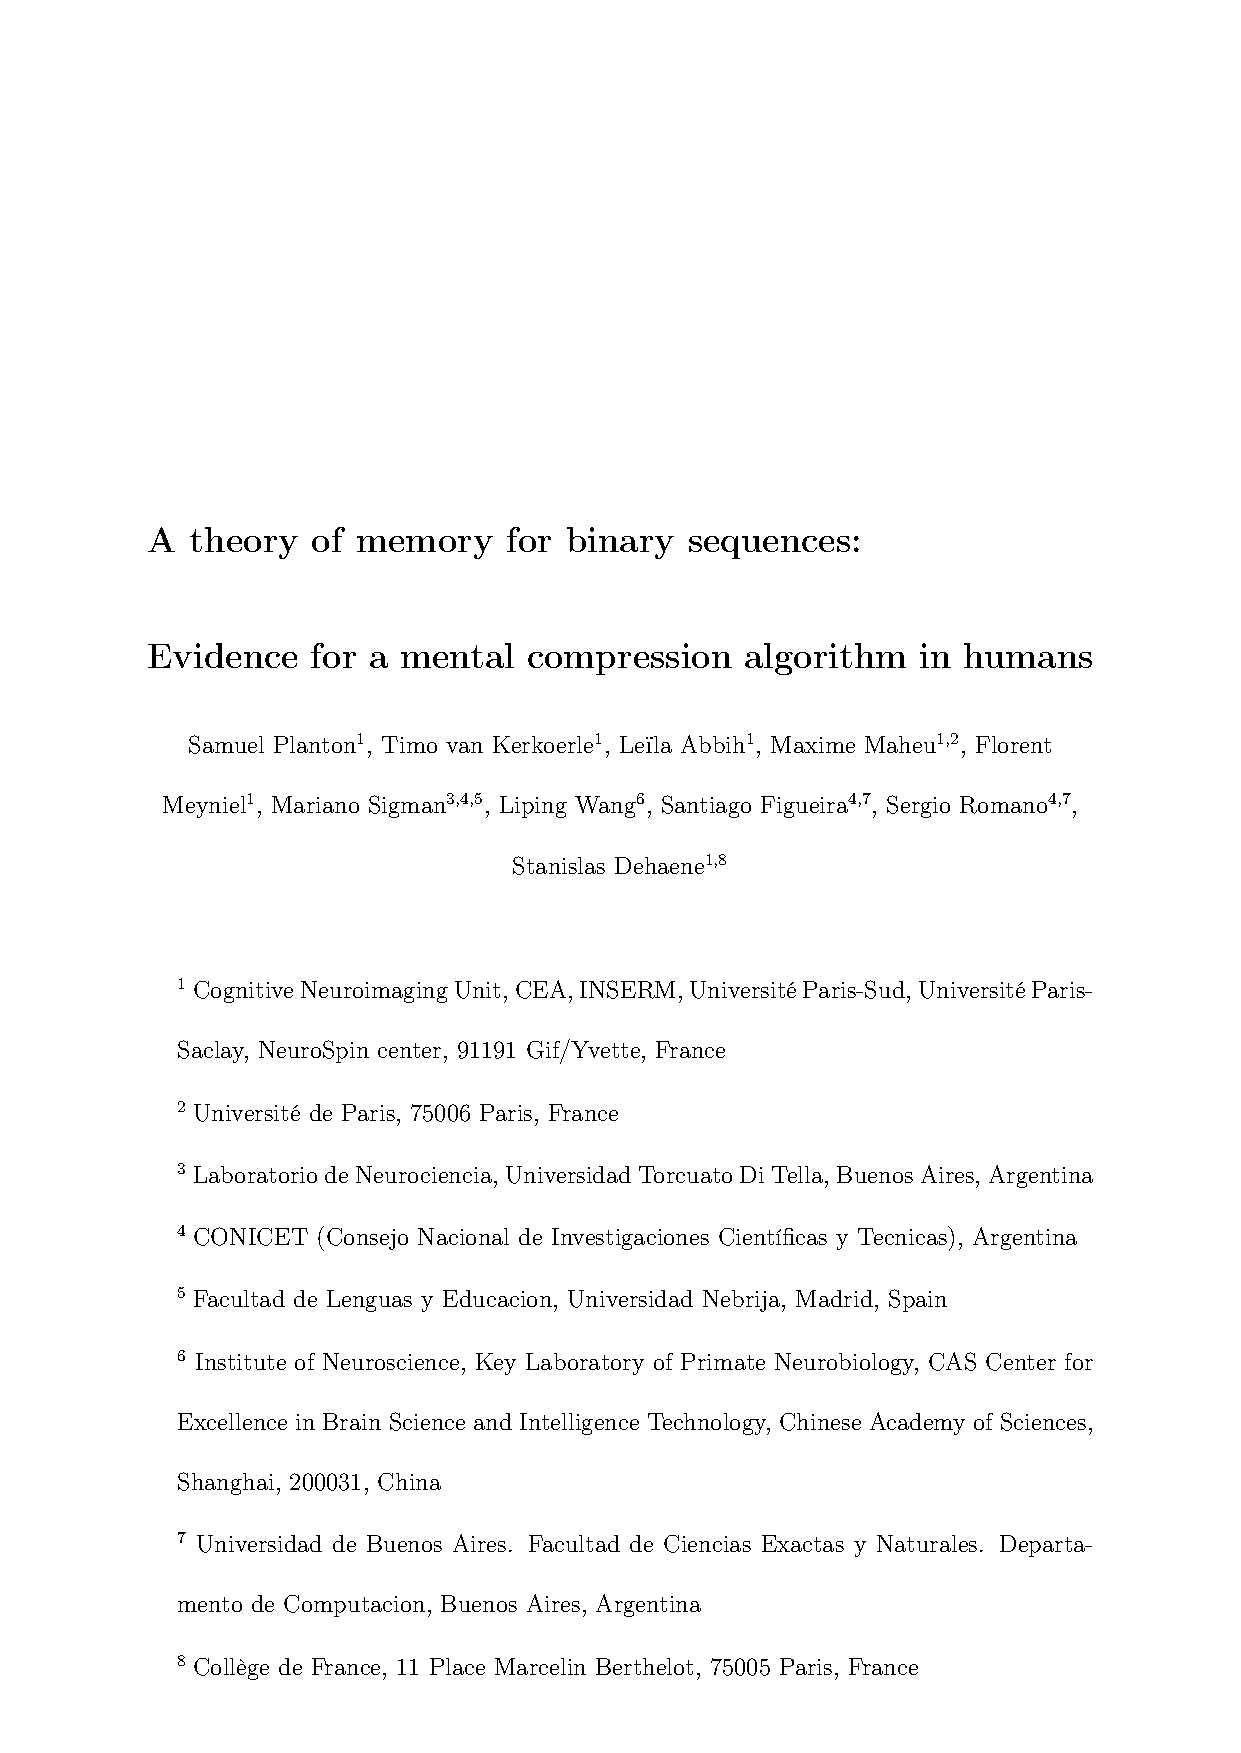
\includepdf[pages=-]{manuscript_pcb.pdf}